\chapter{Theoretische Grundlagen}


\section{Siliziumdetektoren}

Die im Halbleiter vorkommenden Elektronen des Siliziumkristalls wechselwirken mit anderen Elektronen und
Kernen, wodurch es zu vielen Aufspaltungen des Energieniveaus dieser kommt. Die
Zustände liegen dicht bei einander, weshalb von Energiebändern gesprochen wird.
Das höchste von den Elektronen besetzte Band ist das Valenzband, welches von dem
nächsthöheren Band durch eine Bandlücke getrennt ist. Elektronen können
durch Anregungen in das Leitungsband wandern und somit Strom leiten, vorausgesetzt
die Anregungen sind größer als die Energielücke.

Das Einbringen von Fremdatomen in den Siliziumkristall kann dessen Eigenschaften ändern
und wird Dotierung genannt.
Hat das Fremdatom mehr oder weniger Valenzelektronen als das Silizium, kommt
es zu weiteren Aufspaltungen der Energieniveaus, welche sich in der Energielücke
befindet. Dadurch wird es für Elektronen einfacher in das Leitungsband zu wandern.
Bei den Fremdatomen wird zwischen Donatoren und Akzeptoren unterschieden, wobei die
Ersteren mehr Valenzelektronen als das Silizium besitzen und die Zweiteren weniger.
Bereiche des Siliziumkristalls mit Donatoren werden n-Dotierte Halbleiter
und Bereiche mit Akzeptoren p-Dotierte Halbleiter genannt.

Bei einem Übergang von einer n-Dotierten zu einer p-Dotierten Schicht rekombinieren
die Elektronen der n-Dotierten Schicht mit den Elektronenlöchern der p-dotierten Schicht, da beide
in die anderen Bereiche diffundieren. Durch die übrig bleibenden ortsfesten Atomkerne
baut sich ein elektrisches Feld auf, welches dem Diffusionsstrom entgegenwirkt.
Ein sich einstellendes Gleichgewicht führt zu einer raumladungsfreien Zone bei
dem p-n-Übergang.
Für Detektoren werden die eiden Schichten unterschiedlich stark Dotiert, wobei typischerweise
mehr Akzeptoren als Donatoren in den Siliziumkristall eingebracht werden. Bei
asymmetrischer Dotierung breitet sich die Verarmungszone hauptsächlich in die schwächer dotierte Seite aus. 
Durch eine äußere Spannung wird die Zone vergrößert und dient als Ionisationskammer für einfallende Teilchen. Diese streuen
an den Atomkernen in der Zone und geben ein Teil oder ihre gesamte Energie bei dem Durchgang durch den Detektor ab. Mit der so abgegebenen
Energie werden Elektron-Loch Paare erzeugt, welche sich durch das vorhandene elektrische Feld zu ihrer jeweiligen dotierten
Schicht bewegen und über Elektroden als elektrisches Signal gemessen werden können.
Die raumladungsfreie Zone dient somit als Detektor und soll ein möglichst großes Volumen umfassen.

Mehr Informationen über Halbleiter finden sich beispielsweise in dem Buch "Halbleiter-Leistungsbauelemente"  \cite{semiconductor}.

\section{Strahlenschäden}
Wechselwirkungen von hochenergetischen Teilchen mit Silizium können zu Defekten in deren
Gitterstruktur führen.
Die Energie der Teilchen an die Gitteratome wird dabei durch Ionisation und elastischer Streuung abgeben. Die Ionisation der
Gitteratome wird "Total Ionizing Dose" (TID) genannt und führt zu keinen Schäden im Gitter.
Es muss zwischen verschiedenen Arten von Defekten unterschieden werden. Die Teilchen können ein Gitteratom aus dem
Gitter herausschlagen, wodurch eine Leerstelle und ein Zwischengitteratom entstehen. Das herausgeschlagene Atom
kann Silizium, aber auch ein Fremdatom sein. Daraus folgt eine Änderung der Dotierungskonzentration im
Halbleiter und somit eine Änderung seiner Eigenschaften.
Leerstellen können mit Fremdatomen und anderen Leerstellen Bindungen eingehen. Die
entstehenden Komplexe sind stabil und verändern den Halbleiter permanent.

Nach der "Non-Ionizing Energy Loss" (NIEL) Hypothese wird der Detektorschaden durch die Energie des herausgeschlagennen
Atoms beschrieben und ist unabhängig von der ursprünglichen Wechselwirkung.
Um somit Fluenzen $ \Phi$ von verschiedenen Teilchen (Lepton, Hadron) miteinander vergleichen zu können, werden diese
auf eine $\SI{1}{\mega\eV}$ Neutronstrahlung normalisiert und haben die Einheit $\mathrm{\frac{n_{\mathrm{eq}}}{cm^2}}$.


\section{Annealing der Dotierungskonzentration}
Annealing beschreibt allgemein die durch Erhitzung hervorgerufenen Veränderungen von Materialeigenschaften. Für die
Halbleiter sollen dabei, durch die zugeführte Wärme, die Defekte teilweise behoben werden, um somit eine
bessere Funktionsfähigkeit über einen längeren Zeitraum zu garantieren. Die auftretenden Effekte sind dabei wie folgt:

\textbf{1. Migration:} Ist die Temperatur hoch genug können die Zwischengitteratome durch das Gitterwandern und
zum einen Leerstellen im Gitter füllen.

\textbf{2. Komplexformation:} Das Migrieren der Atome kann zum Ausbilden von Komplexen führen. So kann sich zum Beispiel ein
Zwischengittersiliziumatom mit einem Siliziumatom im Gitter binden.

\textbf{3. Dissoziation:} Komplexe können bei hohen Temperaturen Dissoziieren, wodurch einzelne Bestandteile des Komplexes
durch das Gitter migrieren können. Dafür muss die Schwingungsenergie des Gitters größer als die Bindungsenergie der Komplexe sein.

Die Annealingeffekte bewirken eine Änderung in der Dotierungskonzentration $N_{\mathrm{eff}}= |N_{\mathrm{D}}-N_{\mathrm{A}}|$, welches durch das Hamburger Modell beschrieben wird.
Die Änderung von $N_{\mathrm{eff}}$ ist gegeben durch:
\begin{align}
  \Delta N_{\mathrm{eff}}(t, \Phi_{\mathrm{eq}}, T)   = N_{\mathrm{C}}(\Phi_{\mathrm{eq}}) + N_{\mathrm{A}}(t, \Phi_{\mathrm{eq}}, T) + N_{\mathrm{Y}}(t, \Phi_{\mathrm{eq}}, T) \label{eqn:N_eff}
\end{align}
Die einzelnen Summanden werden im folgenden erläutert.

\textbf{\textit{Stable Damage}} $\symbf{N_{\mathrm{C}}}:$ Der stable Damage ist unabhängig von der Temperatur und wird durch das annealing nicht beeinflusst.
\begin{align}
  N_{\mathrm{C}}(\Phi_{\mathrm{eq}}) = N_{\mathrm{C0}}[1-\exp{(-c \cdot \Phi_{\mathrm{eq}})}] + g_{\mathrm{c}} \cdot \Phi_{\mathrm{eq}}
\end{align}
Der erste Summand folgt aus einer unvollständigen Entfernung von Donatoren, der zweite Summand beschreibt stabile Defekte, welche sich wie Akzeptoren verhalten \cite{beyer}.
Hierbei beschreibt $N_{\mathrm{C0}}$ die Amplitude , $g_{\mathrm{c}}$ die sogenannte "introduction rate" der Akzeptoren und $c$ einen Fitparameter.

\textbf{\textit{Shortterm annealing}} $\symbf{N_{\mathrm{A}}}:$ Das shortterm annealing bewirkt eine Verringerung der Dotierungskonzentration und entsteht durch
das Annealing von Akzeptoren, was zu einer kleineren Dotierungskonzentration führt. . Dieser Effekt wird
zur Ausheilung des Sensors verwendet. Die Bezeichnung rührt daher, dass $N_{\mathrm{A}}$ meistens in den ersten 100 Minuten verschwindend gering wird. Die
Funktion wird näherungsweise beschrieben durch:
\begin{align}
  N_{\mathrm{A}}(t, \Phi_{\mathrm{eq}}, T) = \Phi_{\mathrm{eq}} \cdot g_{\mathrm{a}} \cdot \exp{\left(-\frac{t}{\tau_{\mathrm{a}}(T)}\right)}
\end{align}
Mit der Temperaturabhängigen Funktion
\begin{align}
  \tau_{\mathrm{a}}(T) = \frac{1}{k_{0\mathrm{Y}}}\exp{\left(\frac{E_{Y}}{k_{\mathrm{b}}T}\right)}.
\end{align}

\textbf{\textit{Longterm annealing}} $\symbf{N_{\mathrm{Y}}}:$ Der Aufbau von
Akzeptoren sorgen nach einem hinreichend großen Zeitraum für eine steigende
Dotierungskonzentration. Dieser Effekt wird wie folgt berechnet.
\begin{align}
  N_{\mathrm{Y}}(t, \Phi_{\mathrm{eq}}, T)     = N_{\mathrm{Y , \inf}}\cdot \left(1 - \frac{1}{1 + \frac{t}{\tau_{\mathrm{Y}}(T)}}\right)
\end{align}
Beginnend bei null geht diese Funktion nach einem unendlich langen Zeitraum gegen die Konstante $N_{\mathrm{Y, \inf}}$.
Hierbei gilt für $\tau_{\mathrm{Y}}(T)$:
\begin{align}
  \tau_{\mathrm{Y}}(T) = \frac{1}{k_{0\mathrm{a}}}\exp{\left(\frac{E_{aa}}{k_{\mathrm{b}}T}\right)}.
\end{align}

In Abbildung \ref{fig:n_eff_beispiel} ist Beispielhaft das Annealingverhalten eines
Sensors dargestellt.

\begin{figure}
  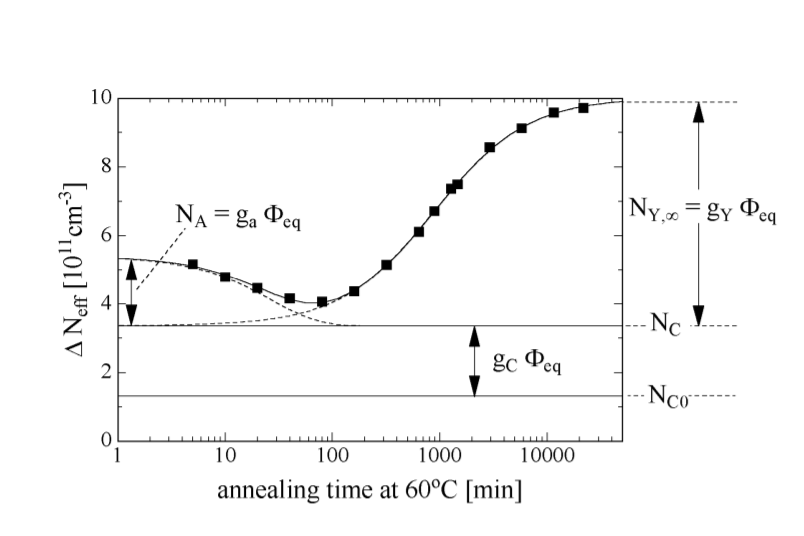
\includegraphics[width=0.95\textwidth]{logos/n_eff_beispiel.PNG}
  \caption{Dotierungskonzentration bei 60°C für eine Bestrahlung mit einer Fluenz
  von $\Phi=\SI{1.4e13}{\per\centi\meter\squared}$ .\cite{moll}}
  \label{fig:n_eff_beispiel}
\end{figure}



\section{Annealing des Leckstroms}
Der Leckstrom beschreibt allgemein einen messbaren Stromfluss über einen als isolierend
angenommenen Weg. Bei Halbleitern ist damit der Strom gemeint, der trotz sperrender
Diode fließt. Dieser entsteht durch die Diffusion von einzelnen Ladungsträgern, welche
in der Realität nicht komplett verhindert werden kann.
Zusätzlich kommt ein Leckstrom durch strahlungsinduzierte Defekte hinzu, welche
Elektronen-Loch-Paare generieren \cite{moll}.
Durch das Annealing kann der Leckstrom somit verringert werden.

Die Fluenz und der durch Strahlung hervor gerufene Leckstrom $\Delta I$ sind
proportional zueinander.


\begin{align}
  \Delta I = \alpha \Phi_{\mathrm{eq}} \cdot V
\end{align}
Hierbei ist $V$ das Volumen des Detektormaterials und $\alpha$ die
sogenannte Schadensrate.
%Der Leckstrom ist vor der Bestrahlung des Sensors
%vernachlässigbar klein im Vergleich zu dem Leckstrom nach der Bestrahlung,
%weshalb $\Delta I$ als Näherung den gesamten Leckstrom beschreibt.

Der Leckstrom vor und nach der Bestrahlung ist temperaturabhängig und wird
beschrieben durch
\begin{align}
  I(T) \propto T^2 \exp{\frac{-E_{\mathrm{g}}}{2 k_{\mathrm{B}}T}} \text{\cite{moll}} \label{eqn:Chilingarov_2013}.
\end{align}
Hier ist $E_{\mathrm{g}}$ die Energie der Bandlücke.

Die Verringerung des Leckstromes durch annealing wird mit der Schadensrate
beschrieben, welche als eine Funktion abhängig von der Zeit und
Temperatur beschrieben wird.\cite{moll}

\begin{align}
  \alpha(t, T) = \underbrace{\alpha_I \cdot \exp{\left(-\frac{t}{\tau_{\mathrm{I}}(T)}\right)}}_{\mathrm{shortterm \: annealing}} + \underbrace{\alpha_{\mathrm{0}}(T) -\beta \cdot \ln{\left(\frac{t}{t_{\mathrm{0}}}\right)}}_{\mathrm{longterm \: annealing}} \text{\label{eqn:damage}}
\end{align}
Mit den in \cite{moll} berechnete Werten für $\alpha_{\mathrm{0}}(T)$:
\begin{align}
  \alpha_{\mathrm{0}}(T) = \SI{-8.9e-17}{\ampere\per\centi\meter} + \SI{4.6e-14}{\ampere\kelvin\per\centi\meter} \cdot \frac{1}{T}
\end{align}

Anders als das Annealingverhalten der Dotierungskonzentration kann die Schadensrate
bei fortschreitendem annealing nur sinken. Für kurze und
lange Zeiten dominieren wie bei der Dotierungskonzentration unterschiedliche
Terme. Für große Temperaturen und Zeiten würde die Schadensrate kleiner als null
werden. Die Messwerte für kleine $\alpha$ weichen jedoch von dem
theoretischen Verlauf ab und nähern sich einen Wert größer null an. Dies
ist in Abbildung \ref{fig:damage_rates} dargestellt.

\begin{figure}
  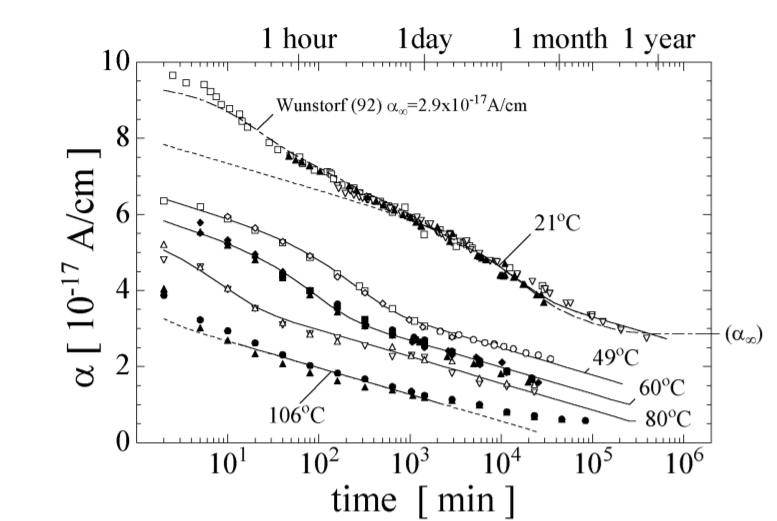
\includegraphics[width=0.9\textwidth]{logos/schadensraten.PNG}
  \caption{Schadensraten für verschiedene konstante Annealingtemperaturen.\cite{moll}}
  \label{fig:damage_rates}
\end{figure}
